\documentclass{exam}
\usepackage{graphicx} % Required for inserting images
\usepackage{amsmath}
\usepackage[left=3cm, right=3cm]{geometry}
\usepackage{multicol}
\usepackage{xcolor}
\usepackage{comment}

\printanswers % If you want to print answers
%\noprintanswers % If you don't want to print answers
% Specifies the way question are displayed:
\qformat{\textbf{Question\thequestion}\quad(\thepoints)\hfill}
\usepackage{color} % defines a new color
\definecolor{SolutionColor}{rgb}{0.8,0.9,1} % light blue
\shadedsolutions % defines the style of the solution environment
% \framedsolutions % defines the style of the solution environment
% Defines the title of the solution environment:
\renewcommand{\solutiontitle}{\noindent\textbf{Solution:}\par\noindent}




\begin{document}

\large{\textbf{Differential equations and the Energy Balance Model (Alternate), Math 100}}


Raphael Kelly, Sven Bachmann, and Peter Harrington

\normalsize
\hrulefill

\

\begin{comment}
\noindent Differential equations form an important part of climate science and have been used to model the Earth's temperature based upon the physical principles involved. This question is split into three major parts that are designed to walk you through some of the questions that you may have as a real applied mathematician and climatologist. Use of online graphing tools, such as Desmos, is encouraged for this problem set. Analytic solutions are required everywhere except where stated otherwise.

\begin{itemize}
    \item Designing and justifying models for real world phenomena is an important part of mathematical research. Part A of this problem encourages you to take the time to understand the motivation behind an important and common climate model and guides you through the analysis of certain aspects of this model.
    \item Another important part of differential equations research is gaining an understanding of the qualitative behaviour of your system under different parameter values. Part B encourages you to extend your understanding of ODEs to new situations and to consider alternate models.
\end{itemize}
Do not be intimidated by the numbers but instead approach each problem thoughtfully and carefully.

\newpage

\section*{Part A}
\end{comment}


The EBM (Energy Balance Model) is an important model in climate research. It suggests that the rate of change in the Earth's temperature is proportional to the difference in the incoming and outgoing rates of energy transfer due to thermal radiation. Consider the following variable definitions.
    
\begin{center}
\begin{tabular}{ l | l | l }
Symbol & Definition & Units \\
\hline \hline
$C$ & Heat capacity of the Earth & $J K^{-1}$\\  
$T > 0$ & Temperature of the Earth & $K$ \\
$E$ & Thermal energy of the Earth & $J$ \\
$P = \frac{d E}{d t}$ & Power & $W=J s^{-1}$ \\
$t>0$ & Time & $s$ \\
%$\alpha(T) \in [0,1]$ & Albedo & unitless \\
%$Q$ & Rate of insolation & $W m^{-2}$ \\
%$\sigma$ & Stefann-Boltzmann Constant & $Wm^{-2}K^{-4}$ \\
%$\epsilon \in [0,1]$ & emitted fraction & unitless
\end{tabular}
\end{center}
The EBM has the form,

$$
C \frac{d T}{d t} = \underbrace{\pi r^2 Q (1-\alpha(T))}_\text{$P_{\rm in}$} - \underbrace{4 \pi r^2 \sigma \epsilon T^4}_\text{$P_{\rm out}$}
$$
which states that the change in the temperature of the Earth is proportional to the difference in the rates of incoming and outgoing energy transfer due to heat per unit time (called "power").
Here $Q$ represents the rate of incoming solar energy reaching the Earth per square meter, $r$ is the radius of the Earth, $\alpha \in [0,1]$ refers to the albedo which measures the proportion of light reaching the Earth's surface that gets reflected away, $\sigma$ is the Stefan-Boltzmann constant with units $W m^{-2} K^{-4}$ and $\epsilon$ refers to the ``emitted fraction" of Earth which is the proportion of Earth's theoretical maximum energy output that is actually radiated away from the surface and into space. Estimates for the above parameters are
$$
\begin{cases}
    C & = 1.0 \times 10^{23} J K^{-1} \\
    r & = 6.3781 \times 10^{6}m \\
    Q & = 1365 W m^{-2} \\
    \sigma &= 5.6704 \times 10^{-8} W m^{-2} K^{-4}.
\end{cases}
$$

In the EBM model, albedo is considered to be a function of temperature. This is because lighter coloured surfaces reflect more light and colder temperatures tend to result in increased snow and ice coverage. A simplified model for the albedo as a function of temperature is $$
    \alpha(T) =
    \begin{cases}
    0.700 & \{T \leq 247K\} \\
    - 0.0114 T + 3.52 & \{247K < T < 282K\} \\
    0.300 & \{T \geq 282K\}.
    \end{cases}
    $$
where the albedo of the Earth is approximately constant at 0.7 below 247K and 0.3 above 282K, and is a linear function of temperature between 247K and 282K.


\subsection*{Questions}

\begin{enumerate}


\item Assume $\epsilon=0.6$ and let $T_{eq}$ denote any steady-state solution to the energy balance model ODE described above.

\textbf{Determine} all values for $T_{eq}$ and whether they are stable, unstable, or neither. Round your answers to whole numbers. It is okay to determine values via a graphical approach as long as any equations which need to be solved for unknown variables are stated and a full explanation of your approach is included. It may also be useful to include a graph.

\textit{Hint:} when searching for a point where $f(x)=g(x)-h(x)=0$ it is often useful to search for intersection points of $g(x)$ and $h(x)$ when they are graphed on the same plot. Also, when solving equations involving piece-wise functions, it is usually best to split it up into its components and consider each individually.




    \item \textbf{Draw} a simple phase line diagram for the energy balance model.. Write ``S'' above each stable steady-state dot, ``U'' above each unstable steady-state dot, and ``N'' above each dot that is neither. No numbers are needed. You will only be marked on the general location and labelling of dots (for each steady-state solution) and the direction of the arrow heads beside them. Use the template below.

    \begin{center}
    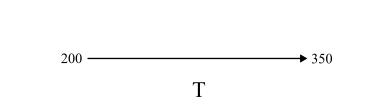
\includegraphics[scale=0.7]{math100phaseline1empty.png}
    \end{center}



    \item We are interested in the behaviour of the system for different values of $\epsilon \in (0,1)$. Let $\epsilon_A < \epsilon_B$ denote two values of $\epsilon$ for which there are exactly two steady-state solutions to the ODE.
    
    \textbf{Find} $\epsilon_A$ and $\epsilon_B$. Use an analytic approach to determine the values to two decimal places.


    \item \textbf{Draw} a typical phase line diagram for the ODE where $\epsilon$ takes on each of the following ranges or values:
    \begin{multicols}{3}
    \begin{enumerate}
        \item $\epsilon \in (0,\epsilon_A)$
        \item $\epsilon = \epsilon_A$
        \item $\epsilon \in (\epsilon_A, \epsilon_B)$
        \item $\epsilon = \epsilon_B$
        \item $\epsilon \in (\epsilon_B, 1)$.
    \end{enumerate}
    \end{multicols}
    As before, write ``S'', ``U'', or ``N'' to indicate the stability of the steady-state. No numbers are needed, but in addition to the location/labelling of dots and the direction of the arrow heads beside them, you will also be marked on the relative location of steady-state dots to those on different phase lines. Use the template below.

    \begin{center}
    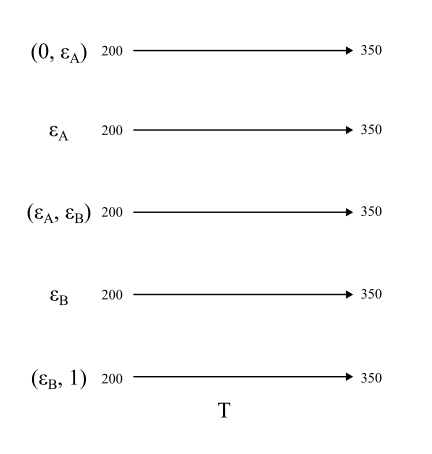
\includegraphics[scale=0.7]{math100phaseline2empty.png}
    \end{center}


    \item Consider an integer-valued function $N(\epsilon)$ which is equal to the number of solutions to the EBM for different values of $\epsilon \in (0,1)$. \textbf{Determine} all values of $\epsilon$ for which $N(\epsilon)$ is discontinuous.



    \item A very generalized relationship exists between $\epsilon$ and $CO_2$ concentration in the atmosphere whereby an increase in atmospheric $CO_2$ leads to a decrease in the value of $\epsilon$. The term equilibrium is used to denote a value of $T$ corresponding to a steady-state solution. 
    
    %If the Earth were to initially have a temperature of $289K$, what would be the effect of increasing atmospheric $CO_2$ concentration on the temperature of the Earth according to this model?
    
    Suppose that at some point in time, $\epsilon > \epsilon_B$ and the Earth's temperature is at a stable equilibrium.  If the the atmospheric $CO_2$ slowly increases and so $\epsilon$ slowly decreases, will the Earth's steady state temperature, $T$ \textbf{increase of decrease}? Assume that the change in $CO_2$ is much slower than it takes for the EBM to reach equilibrium.
    
    \textbf{For what value(s)} of $\epsilon$ is there a discontinuous change in the Earth's equilibrium temperature?



    \item \textcolor{blue}{This question could be skipped to shorten assignment}  Currently, the expression for $P_{out}$ is based upon the assumption from physics that Earth emits like a black-body. However, satellite data has observed an approximately linear relationship between surface temperature and heat emitted by the Earth. In the 1960s, the climate researcher Budyko suggested the alternative expression $P_{out}=4 \pi r^2 \left(A + B T \right)$ where $A=-367.6 Wm^{-2}$ and $B=2.09Wm^{-2}K^{-1}$ were later fitted from data.
    
    \textbf{Draw} a phase line diagram for this new model, using the template below. What value(s) of $\epsilon$ from the previous model yield the same behaviour as this model?

    \begin{center}
    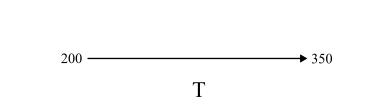
\includegraphics[scale=0.7]{math100phaseline1empty.png}
    \end{center}


    
\end{enumerate}

\noindent What you have done above, analyzing the behaviour of an ODE under different parameter values, is an important part of the mathematical analysis of differential equations. Determining the values of parameters which lead to discontinuous changes in important aspect of an ODE model (such as the number of steady-state solutions) is called bifurcation analysis.

\end{document}